
%(BEGIN_QUESTION)
% Copyright 2011, Tony R. Kuphaldt, released under the Creative Commons Attribution License (v 1.0)
% This means you may do almost anything with this work of mine, so long as you give me proper credit

Two technicians, Jill and Bob, work on programming Siemens S7-200 PLCs to control the starting and stopping of electric motors.  Both PLCs are wired identically, as shown:

$$\includegraphics[width=15.5cm]{i03674x01.eps}$$

However, despite being wired identically, the two technicians' PLC programs are quite different.  Jill's program uses {\it retentive coil} instructions (``Set'' and ``Reset'' coils) while Bob's uses a ``seal-in'' contact instruction to perform the function of latching the motor on and off:

$$\includegraphics[width=15.5cm]{i03674x02.eps}$$

Explain how both of these PLC programs function properly to control the starting and stopping of the electric motor.

\vskip 20pt \vbox{\hrule \hbox{\strut \vrule{} {\bf Suggestions for Socratic discussion} \vrule} \hrule}

\begin{itemize}
\item{} It is ordinarily a bad thing to assign identical bit addresses to multiple coil instructions in a PLC program.  With Jill's retentive coil program, however, this is not only permissible but in fact necessary for its proper operation.  Explain why this is.
\item{} A common misconception of students first learning PLC programming is to think that the type of contact instruction used in the PLC program must match the type of switch contact connected to that input (e.g. ``A N.O. PLC instruction must go with a N.O. switch'').  Explain why this is incorrect.
\item{} Explain how both PLC programs will react if both the ``start'' and ``stop'' pushbuttons are simultaneously pressed.
\item{} Alter both PLC programs to be ``fail-safe'' (i.e. shut the motor off) if ever the stop pushbutton switch fails circuit open.
\end{itemize}

\underbar{file i03674}
%(END_QUESTION)





%(BEGIN_ANSWER)

 
%(END_ANSWER)





%(BEGIN_NOTES)

Jill's program uses retentive coil instructions (Set and Reset), while Bob's program uses standard coil instructions.

%INDEX% PLC, ladder logic program analysis and explanation

%(END_NOTES)


